The problem of taxonomy classification of product titles is central to an e-commerce organization. 
Large online e-commerce companies usually obtain millions of new listing feeds per month from several hundred merchants subscribed to use proprietary ``publish $\rightarrow$ search $\rightarrow$ buy'' platforms specific to each of these companies. 
The ease of use, control on data quality and organization and functionality of these platforms are the key factors for differentiating the success of the revenue generation model for the companies.

The sale of product listings within an e-commerce platform is critically dependent upon end users being able to search for the correct product using some minimal to advanced search functionality provided by the developers of the platform. 
In this paper we differentiate products from product listings using a simple example. 
Consider a product with a title of ``\textit{Wilson tennis racket Level 3 signed by Federer}''. 
Merchant \textbf{A} can list this product with a title of ``\textit{Wilson tennis racquet Level 3 Roger Federer}''' and with a list price of \$80 while merchant \textbf{B} can list the same product with its original title but with a list price of \$72.
The e-commerce platform keeps track of these two product items as two different listings although they are the same product after some title text disambiguation.
Similar examples occur in thousands for product titles having the same title text but differing in price and/or other fields.
Title text disambiguation in absence of any global identifier for products is also a core-problem in e-commerce platforms that follow an online marketplace model, but we do not address that problem here.
In this paper, we will refer to product listings as listings henceforth. 

Most e-commerce companies keep track of high Gross Merchandise Sales (GMS) products and tune search results to queries conditional on GMS and other meta features such as clickstream as well as  content specific features.
One such critical meta feature is the taxonomy classification of listings.
On a web search platform, categories of search results have already been used to improve web query classification \cite{Ganti10} and such kind of query classifications are also very useful for product search engines.
Further, clues from taxonomies have are very useful in user persona detection and targeted campaigns, recommendations, clustering of  ranked lists of listings and many other applications.

\begin{figure}[ht]
	\centering
	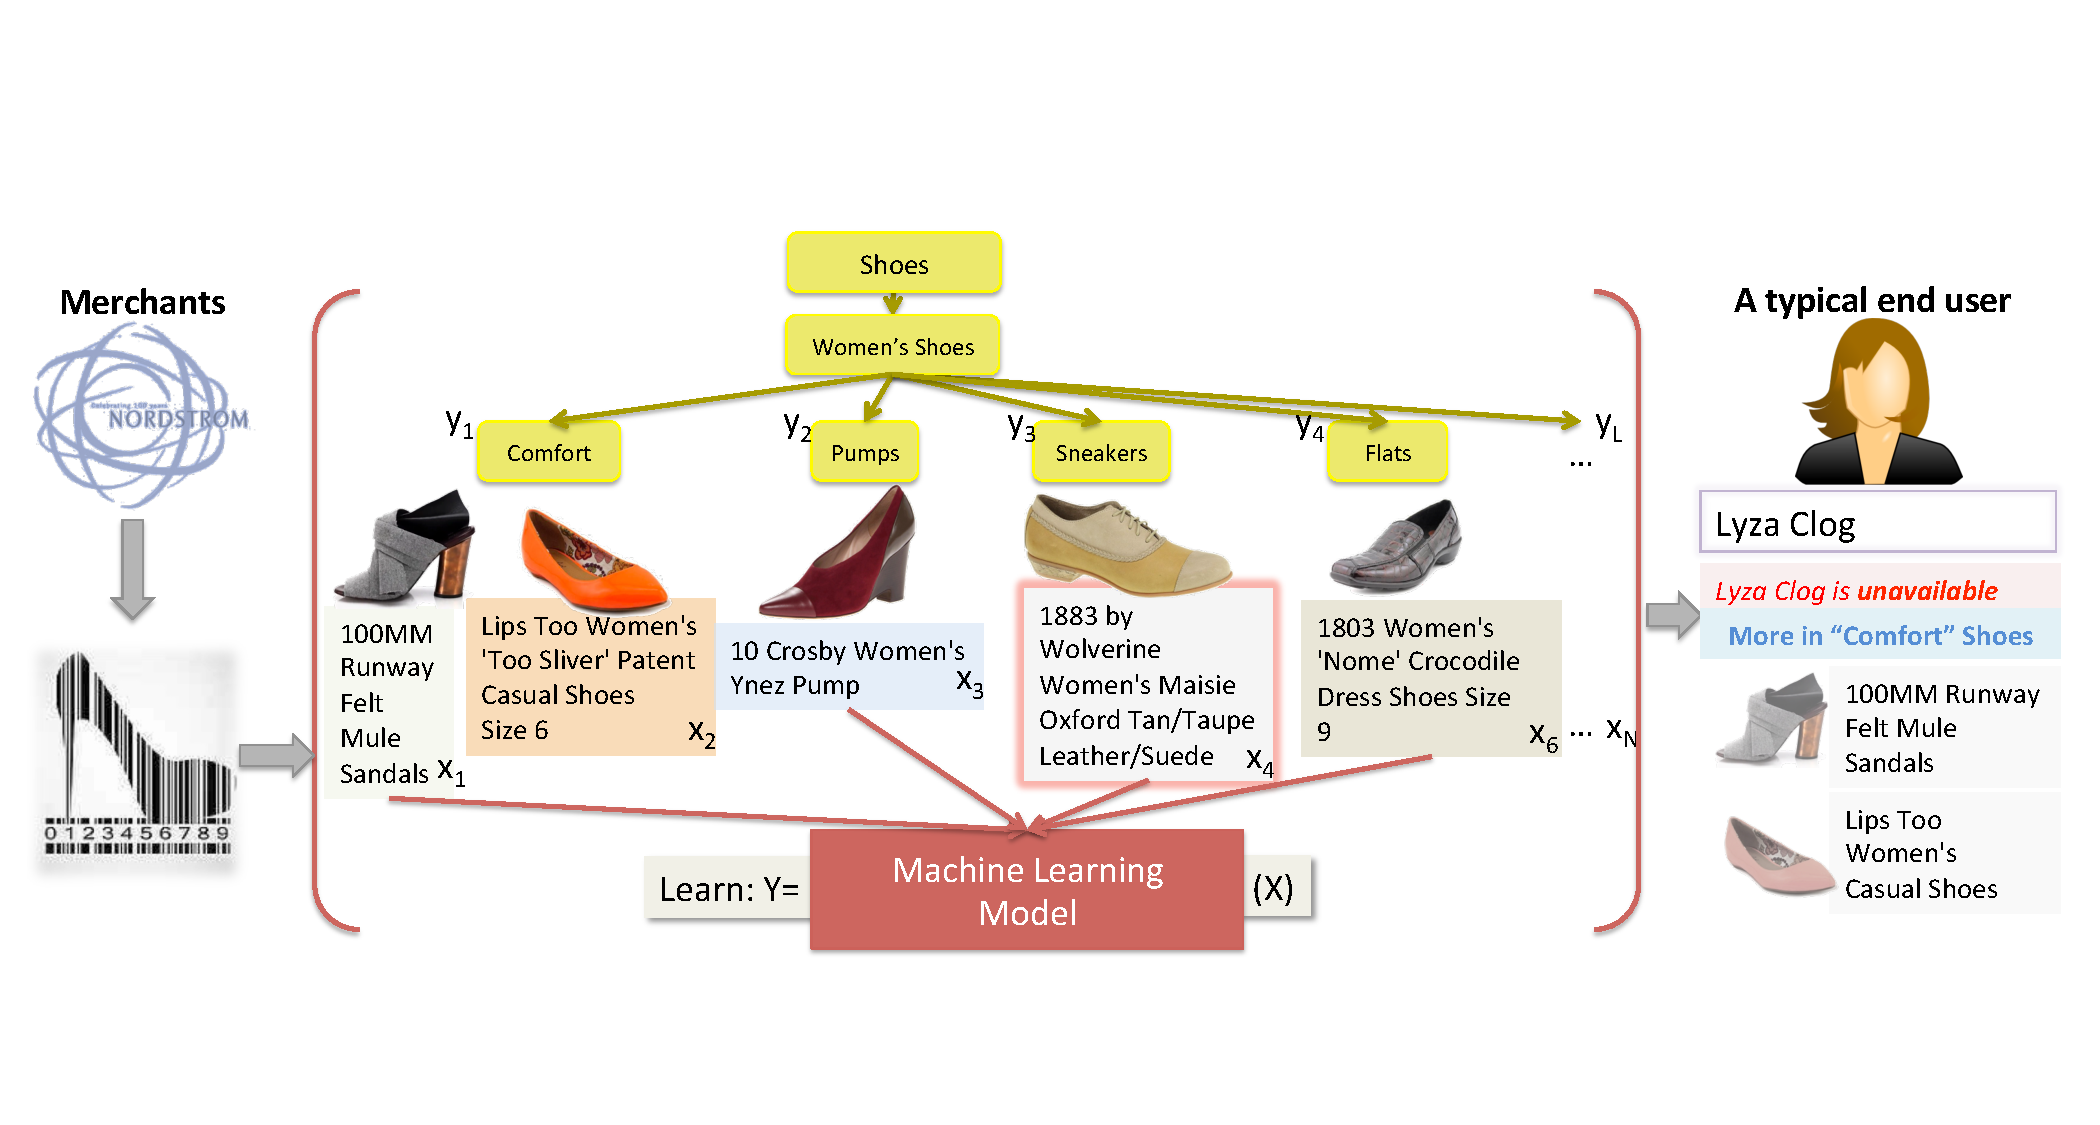
\includegraphics[width=0.9\textwidth]{images/push-pull}
	\vspace{-0.2cm}
	\caption{{\small Merchants push new listings to a data organization and search platform. The listings are then annotated in various ways including a core taxonomy categorization component. The indexed listings together with the annotations influence search and other data organization algorithms. The relevance of the information that end users pull from the indexing platform determines the eventual conversion and revenue generation effectiveness of the e-commerce platform. In this example, it can be easily observed how taxonomy classification can be very helpful in identifying the intent of the query.}}
	\label{Fig:push-pull}
\end{figure}
\vspace{-0.5cm}

In this paper, we focus on taxonomy classification of listings in order to solve problems arising in the scenario described in Fig. \ref{Fig:push-pull}.
Generally, merchants interested in publishing their listings to an online e-commerce platform, pushes their feed to an intelligent indexing engine which then are ready to be consumed by the end user in a variety of ways.
Scalable and accurate taxonomy categorization of listings is often among the earliest core annotation steps for these platforms.
Feeds usually come in at 10-20 million listings/day for mid scale e-commerce companies.

Our problem here is to classify each test instance (listing), $\bm{x}_m$ in Fig. \ref{Fig:push-pull}, into the correct taxonomy branch, $\bm{y}_l$ e.g. ``\textit{Shoes $\rightarrow$ Women's Shoes $\rightarrow$ Comfort}''.
In order to reduce classification calls at runtime and to prevent error snowballing effect of a truly cascading hierarchical classifier, we solve the taxonomy classification problem as a bi-level problem.
For example, a test listing is first classified into one of the level one classes shown in the Fig. \ref{Fig:push-pull} e.g. ``\textit{Shoes}''.
It is then classified by the classification model corresponding to the level one taxonomy subtree identified by the predicted level one root node (e.g. ``\textit{Shoes}'').
As noted in \cite{Julian15}, not all listings reside in leaf nodes, however, for our case, we consider $\bm{y}_l$ to be the label of the node where $\bm{x}_n$ resides, up until the root node of the taxonomy tree.
Empirically, it has been observed that this scheme works best for taxonomies which are at-most four to five levels deep and the total number of branches for the subtrees to less than 200. 

In large e-commerce companies that follow the marketplace models of business to business to customer (B2B2C) commerce, such as Rakuten, maintaining an unified product taxonomy a.k.a product catalog is very difficult. 
This can happen for many reasons including cross-border trading and more importantly acquisitions of external companies that are niche.
Each of the acquired companies has their own taxonomies and although they are merged under a common parent company, they operate as independent Business Units (BUs)  for some time with their own data feeds and data organization algorithms.
In this paper, we perform experiments on listings data from two such BUs -- BU1 and BU2 -- belonging to Rakuten USA Inc.
that is managed by Rakuten Ichiba, the largest e-commerce company in Japan.

Dataset characteristics vary substantially from BU to BU.
In our experiments, we found that data from BU1 is substantially corrected using large scale human annotation efforts to create rules for categorization which are contracted to BU1 only.
This leads to lower coverage at the expense of high precision and much lower noise, however, such kind of manual efforts are not scalable.
On the other hand, the listing feed which BU2 receives is from external data vendors who sell their feed at substantial subscription rates. 
However, the taxonomies and categorization these vendors provide are often wrong.
BU2 converts taxonomies from these data vendors to their own manually and hence directly maps listings without any error correction.
We observe such instances of error in Fig. \ref{Fig:push-pull} for the leaf node ``\textit{Sneakers}'' and the listing ``\textit{1883 by Wolverine Women's Maisie Oxford Tan/Taupe Leather/Suede}'' - the correct leaf node should have been ``\textit{Other} $\rightarrow$ Women's Shoes'' (not shown in Fig. \ref{Fig:push-pull}).

The absence of a ground-truth training set from BU2 constrains us to rely on this noisy dataset for training our classifiers. 
In an industrial setting, automatic categorizations are continuously eliminated manually either in-house (low budget) or through external organizations such as CrowdFlower\footnote{\scriptsize{\url{https://www.crowdflower.com/crowdflower-attacks-data-scientists-biggest-challenge-incomplete-messy-data/}}}.
Needless to mention, the amount of this kind of ``label flip'' error is not nominal and it is hard to correct without manual scans of millions of listings -- an impossible task which is mitigated to some extent for BU2's dataset using topic model based noise analysis (Section \ref{Subsect:BU2-noise-analysis}).


\begin{wrapfigure}{r}{0.42\textwidth}
	\centering
	\vspace{-0.5cm}
	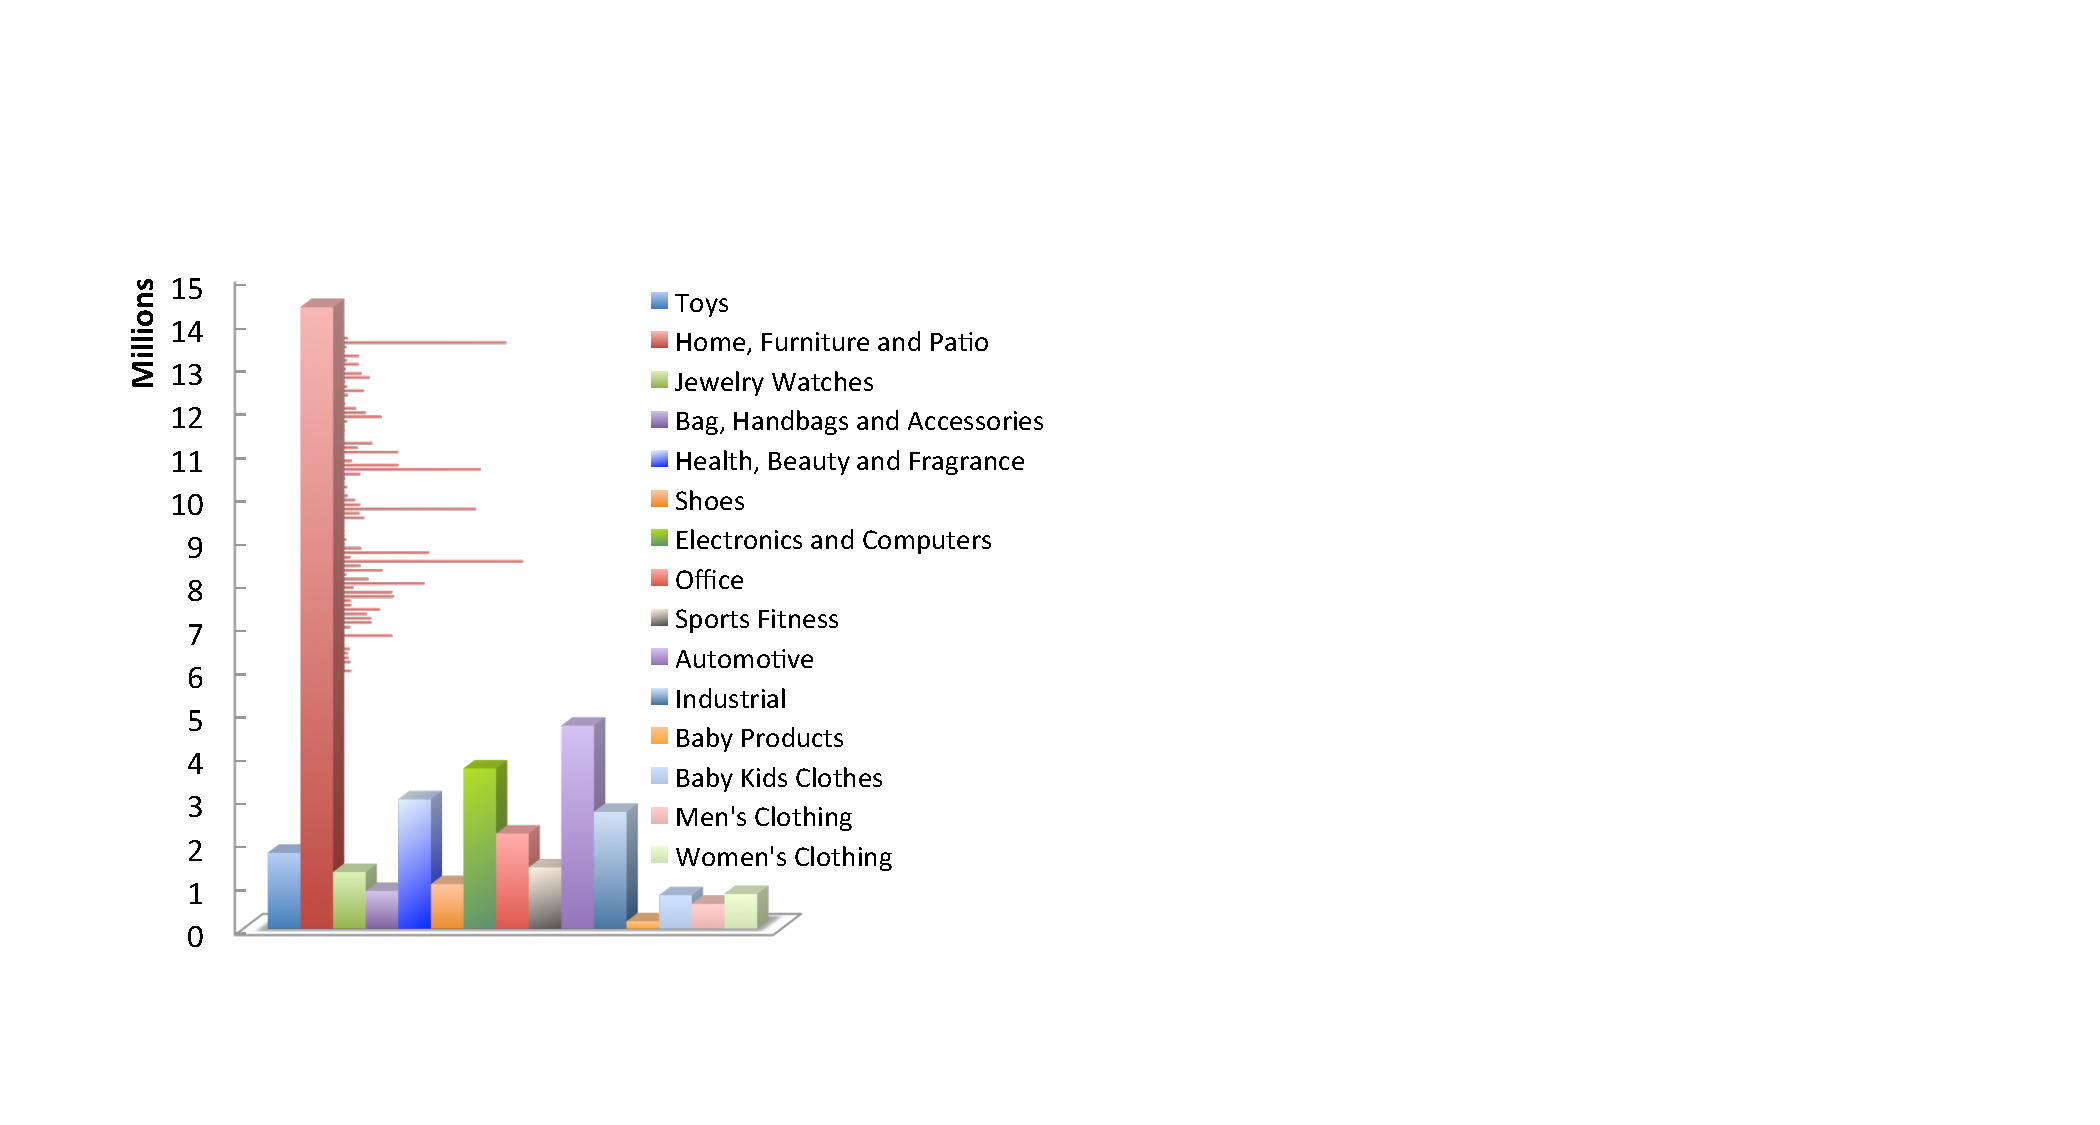
\includegraphics[width=0.42\textwidth]{images/BU2-dataset-Dec2015}
	\vspace{-0.6cm}
	\caption{{\small Dataset from BU2 -- Dec 2015 snapshot. Total number of de-duplicated listings is 40 million.}}
	\vspace{-0.5cm}
	\label{Figure_BU2-datset-earlier}
\end{wrapfigure}
Dataset imbalance is also a major problem in product listing datasets for building classification models.
Most loss functions that are not resistant to imbalance generalize very poorly without resorting to any subsampling techniques \cite{Chawla02:SMOTE}. 
We, instead, resort to cross-entropy (logistic) loss functions which are more resistant to imbalance particularly with suitable regularizers (Section \ref{Sect:results}). 
A preview of the imbalance in BU2's dataset is shown in Fig. \ref{Figure_BU2-datset-earlier} where a disproportionate number of listings appear in the ``Home, Patio and Furniture'' category.
In the experiments shown in Section \ref{Sect:results}, we use BU2's data snapshot from Feb 2016 which initially consists of 204 million deduplicated listings from 277 merchants, dropping down to 60 million after aggressive cleanup (Section \ref{Subsect:BU2-noise-analysis}).


\begin{wrapfigure}{l}{0.45\textwidth}
	\centering
	\vspace{-0.6cm}
	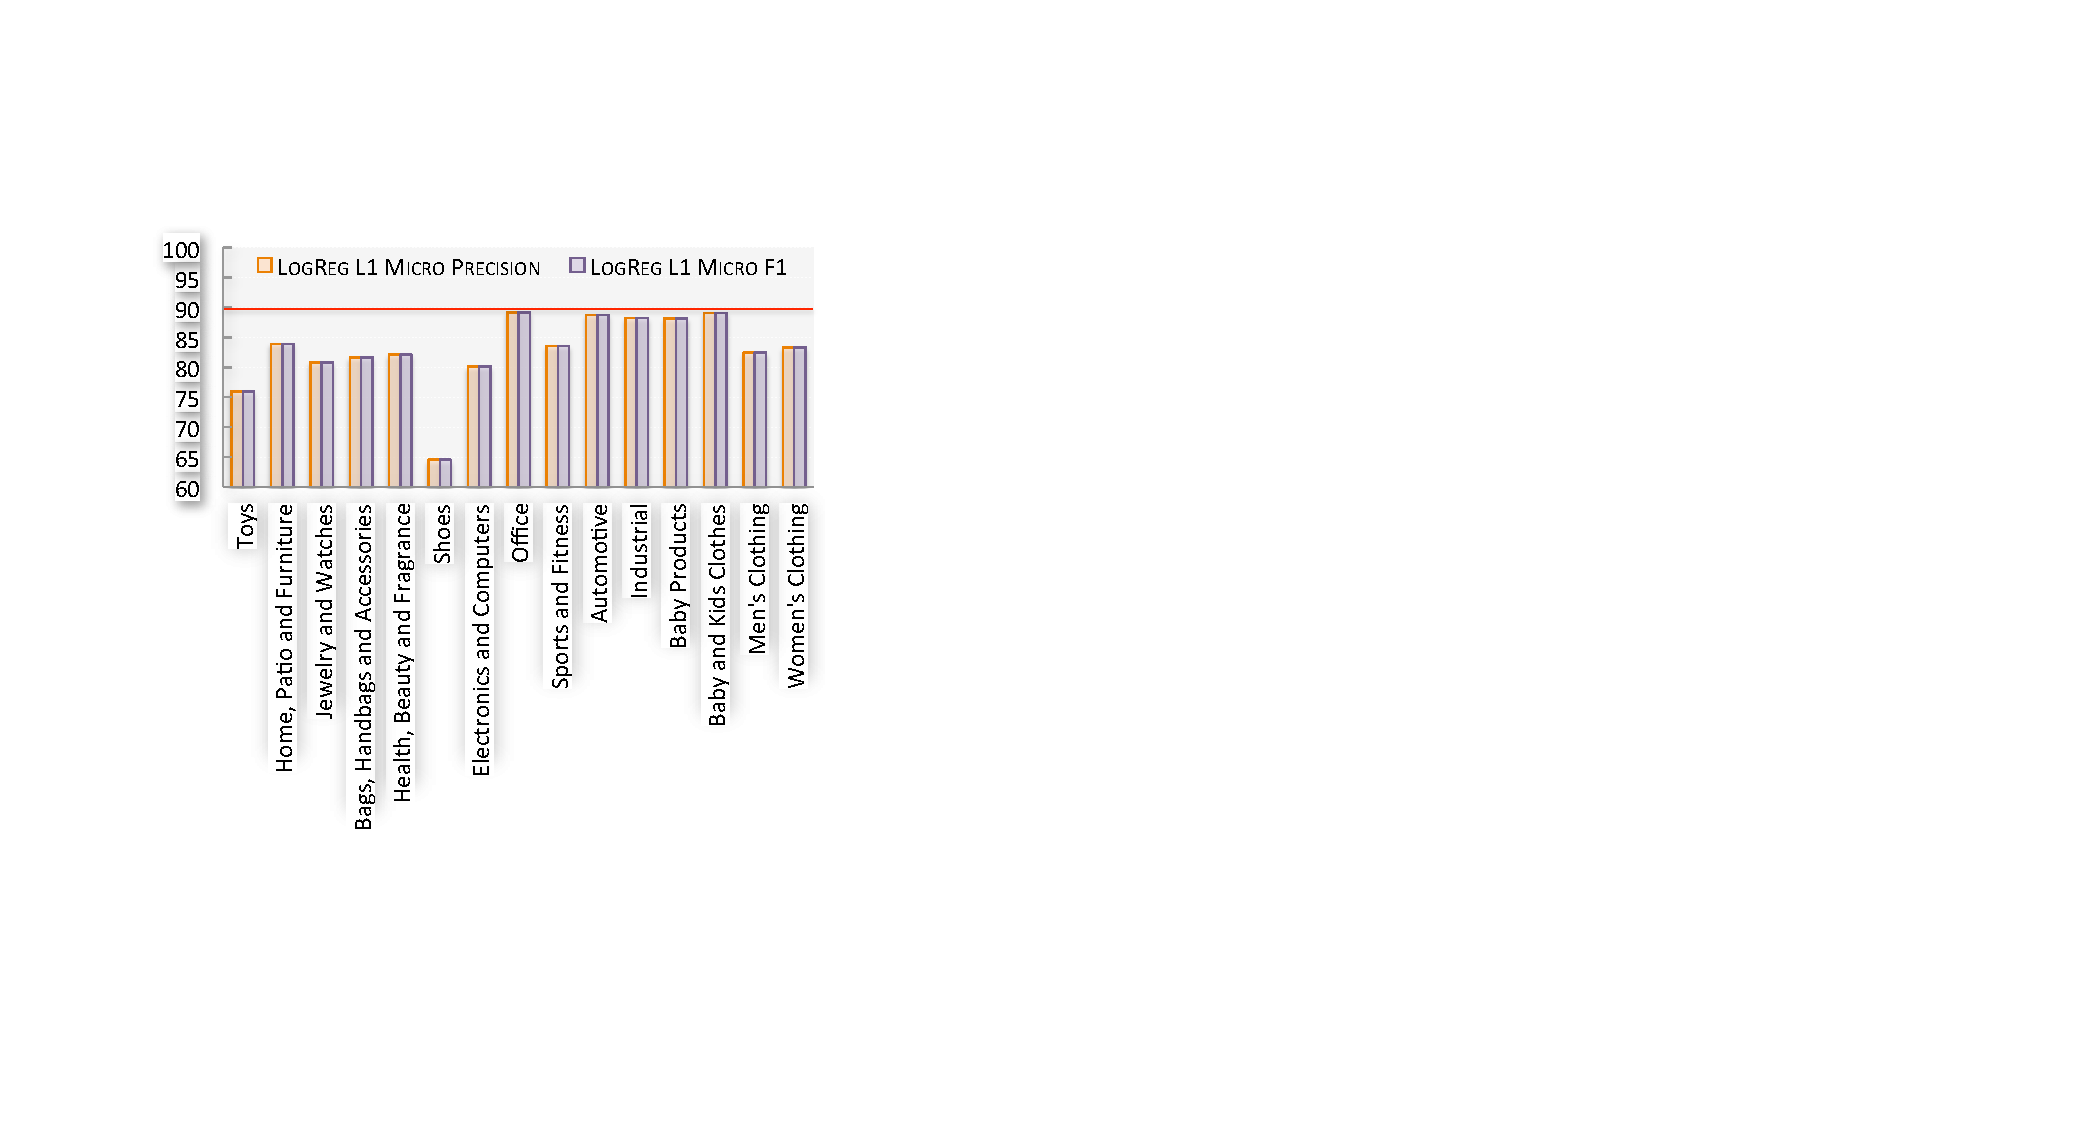
\includegraphics[width=0.45\textwidth]{images/BU2-Dec2015-LogRegL1}
	\vspace{-0.7cm}
	\caption{{\small Micro precision and micro F1 across 15 top level categories obtained using 10\% of the 40 million listings as test set for the dataset in the left }}
	\label{Figure_BU2-WUC-LogRegL1}
	\vspace{-0.5cm}
\end{wrapfigure} 
Our initial experiments using the noisy data in Fig. \ref{Figure_BU2-datset-earlier} using a one vs. one logistic regression model with L1 regularization \cite{Yu13:EBay,LibShortText} show promising results but they do not attain a business requirement of $90\% \pm \epsilon$  mean micro precision across the level one taxonomies.
Logistic Regression (henceforth LogReg) with L1 achieves 83\% mean micro precision (F1 values differed only in the third decimal place) for 10\% test dataset consisting of 4 million listings.
The level zero classification is a much easier problem and most classifiers achieve 90\% micro precision and F1 for all of the datasets considered here with Gradient Boosted Tree (henceforth GBT) \cite{Friedman:GBT} and Convolutional Neural Networks (henceforth CNN) \cite{Kim14} performing the best with 92\%--94\% micro precision and micro F1s. 
Taxonomy classification of the listings in the branches of the ``Shoes'' taxonomy subtree has been very poor and this resulted in a novel way to identify the pattern of noise in whole of BU2's data using unsupervised modeling and minimal manual analysis (Section \ref{Subsect:BU2-noise-analysis}).

\begin{figure}[h]
\centering
	\subfloat[{{\footnotesize BU1 dataset: Total subtrees with taxonomy - 16; Total listings in these subtrees - 12.61 million; Pearson correlation coeff. for branches vs. listings - 0.643 }}]{\label{Fig:BU1-branches+KL}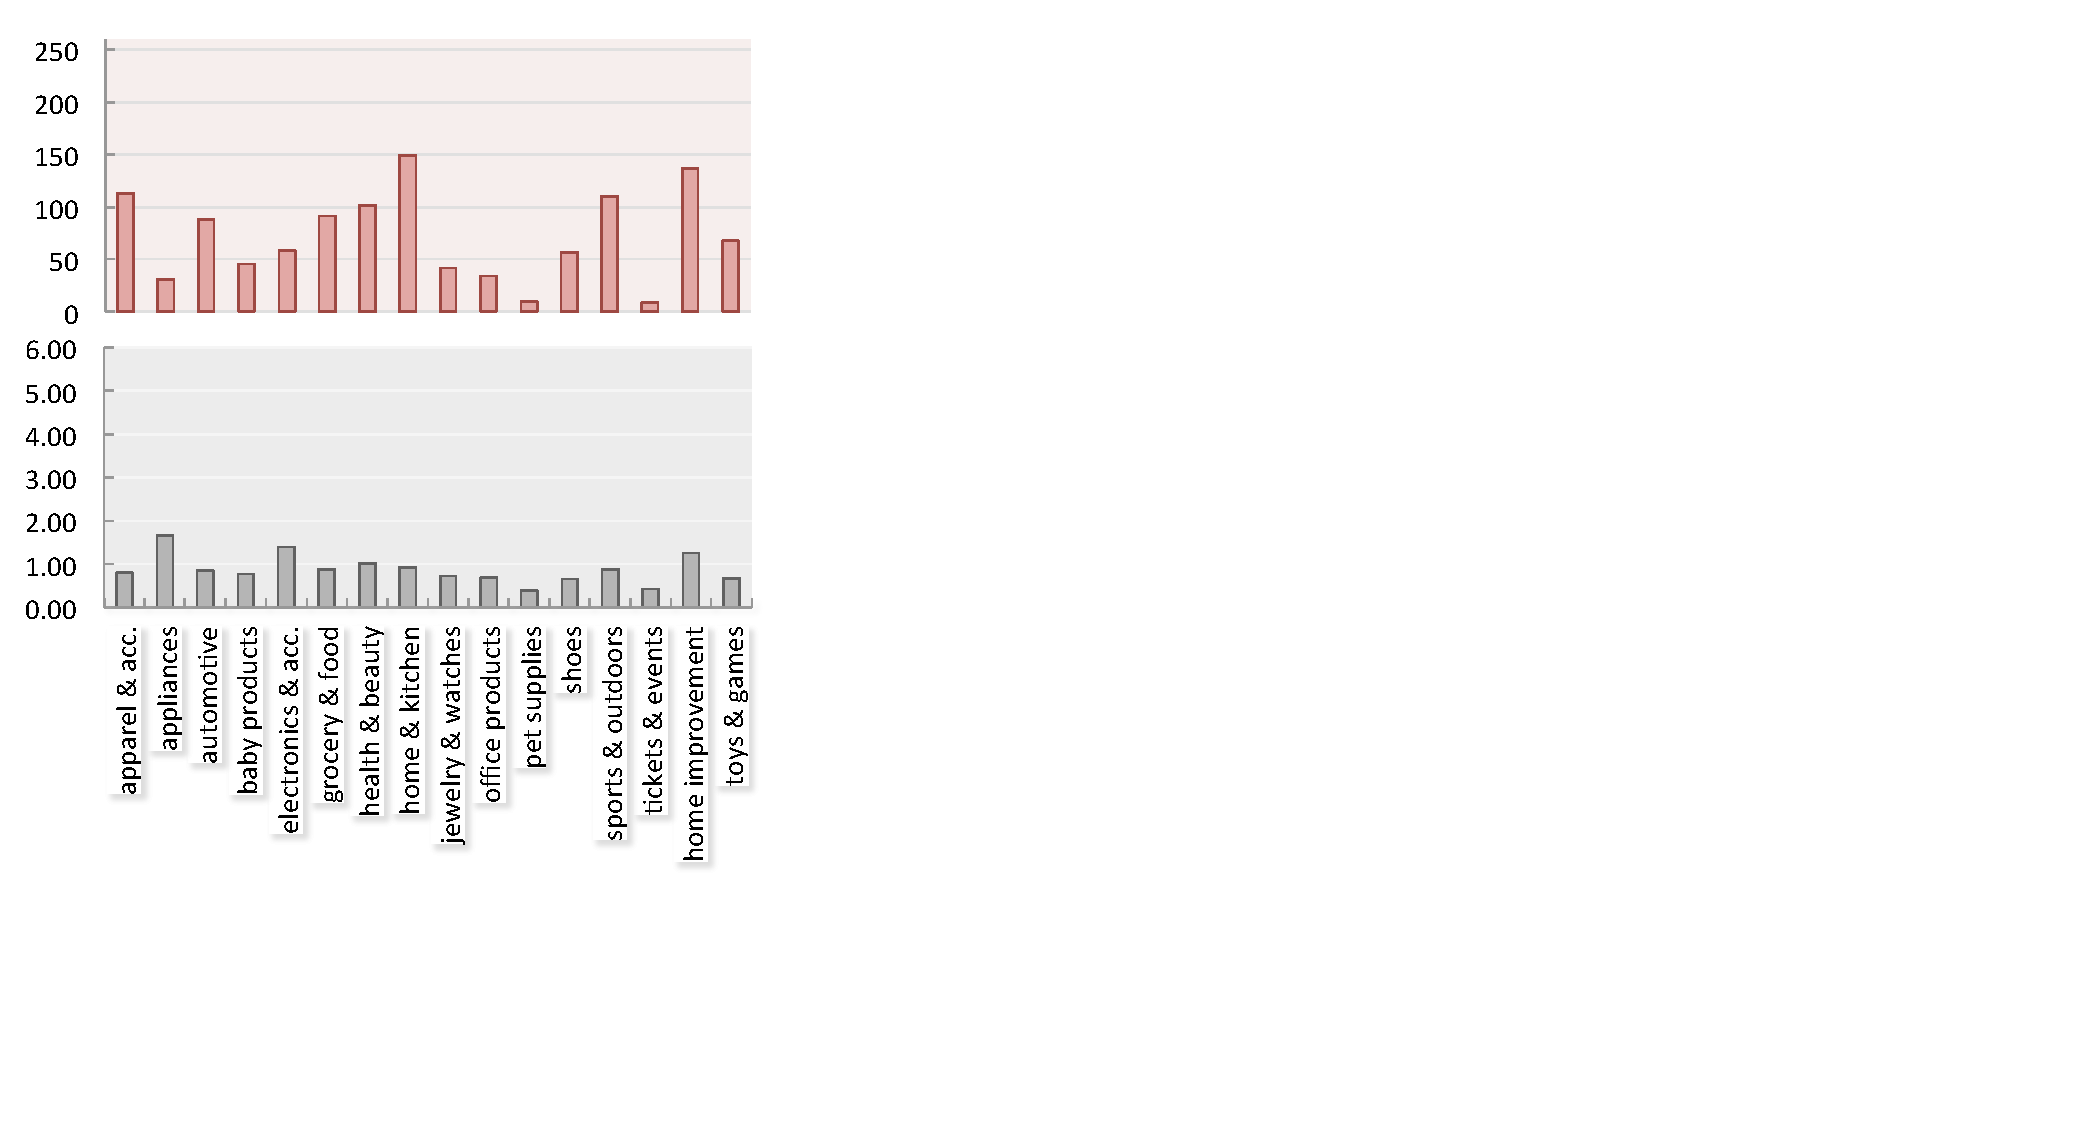
\includegraphics[width=0.3\textwidth]{images/BU1-branches+KL}} \hspace{0.1cm}
	\subfloat[{{\footnotesize AmazonJulian dataset: Total subtrees with taxonomy - 25; Total listings in these subtrees - 7.46 million; Pearson correlation coeff. for branches vs. listings - 0.269}}]{\label{Fig:amazonj-branches+KL}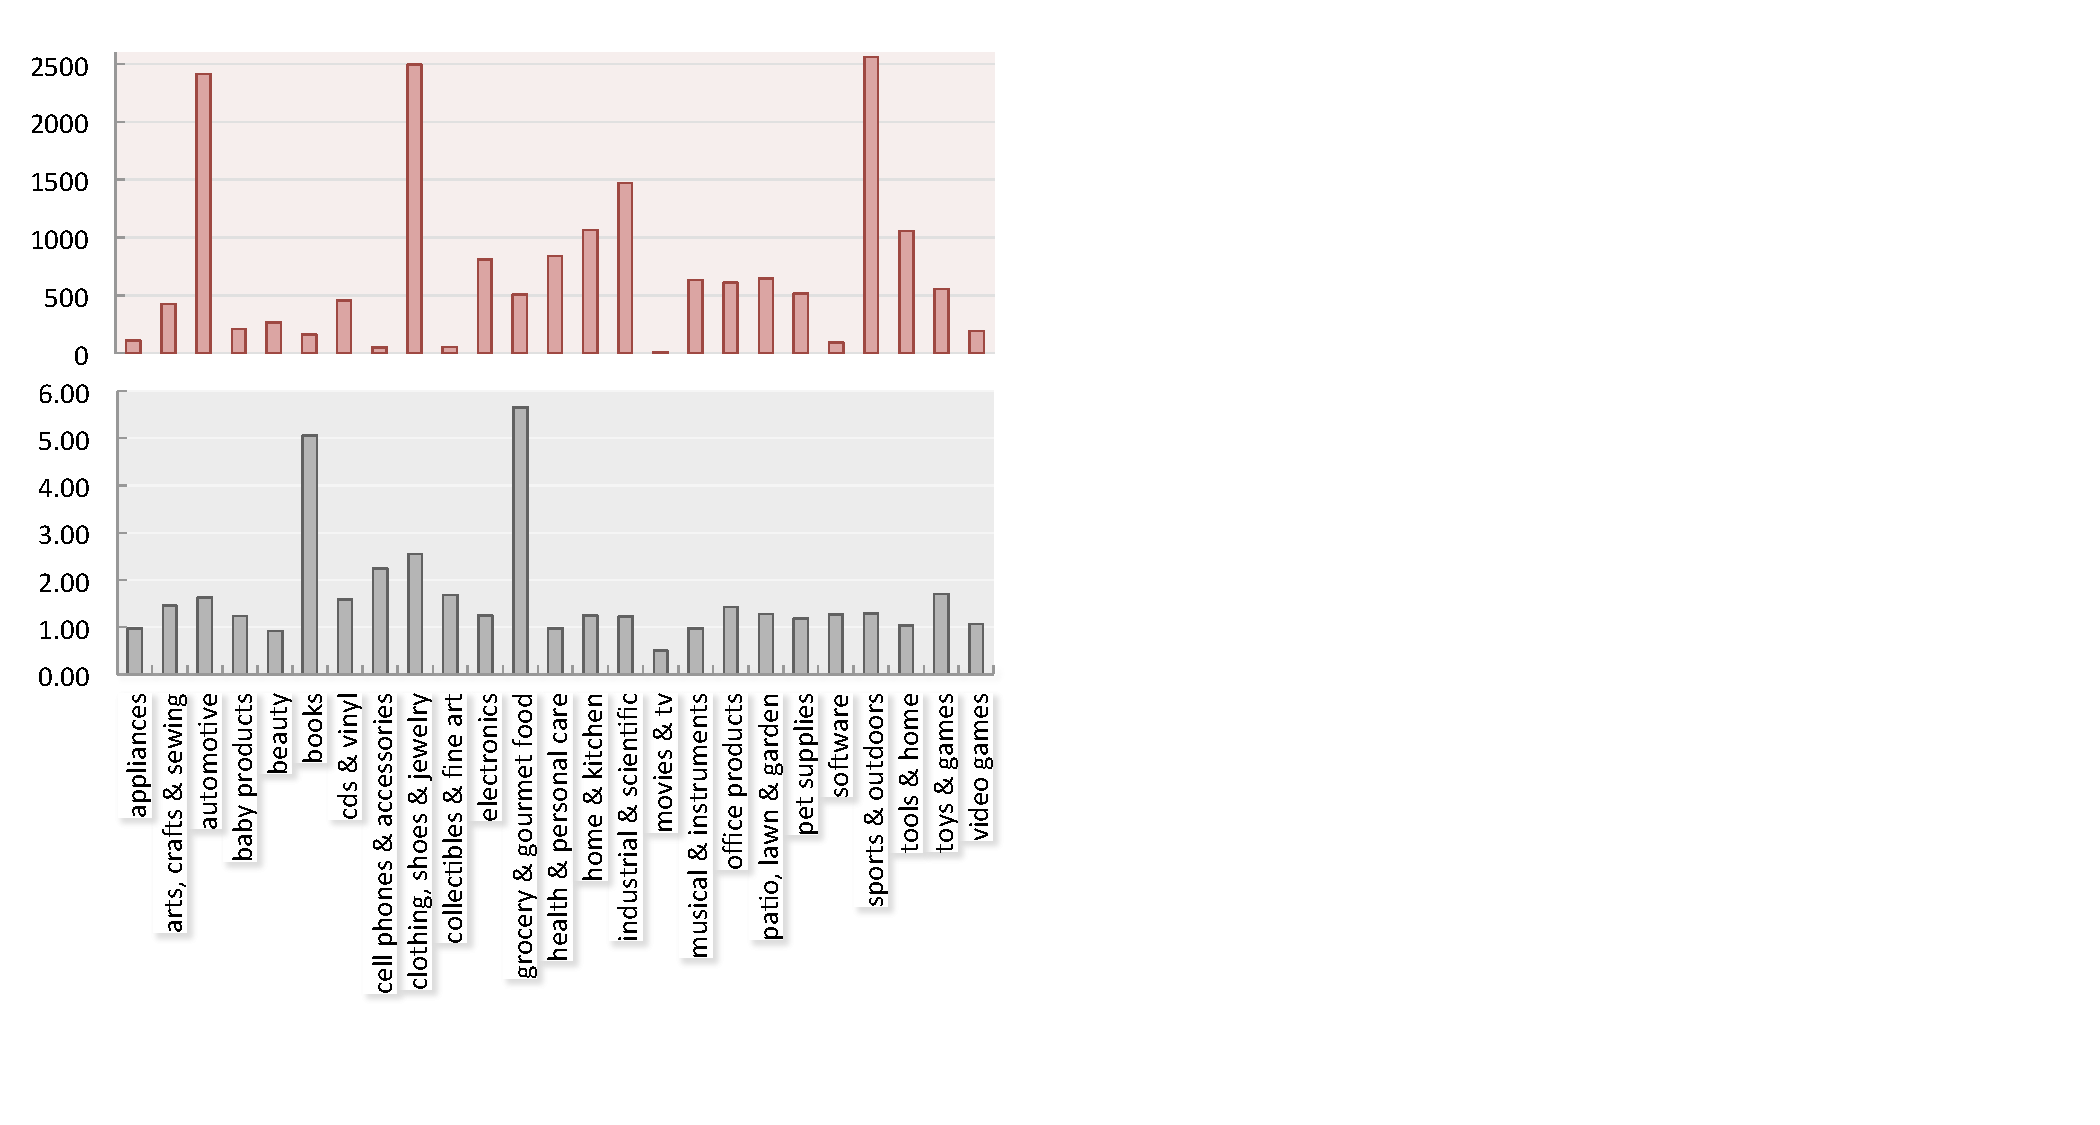
\includegraphics[width=0.37\textwidth]{images/AmazonJulian-branches+KL}} \hspace{0.1cm}
	\subfloat[{{\footnotesize BU2 dataset: Total subtrees with taxonomy - 15; Total listings in these subtrees - 60 million; Pearson correlation coeff. for branches vs. listings - 0.209}}]{\label{Fig:BU2-branches+KL}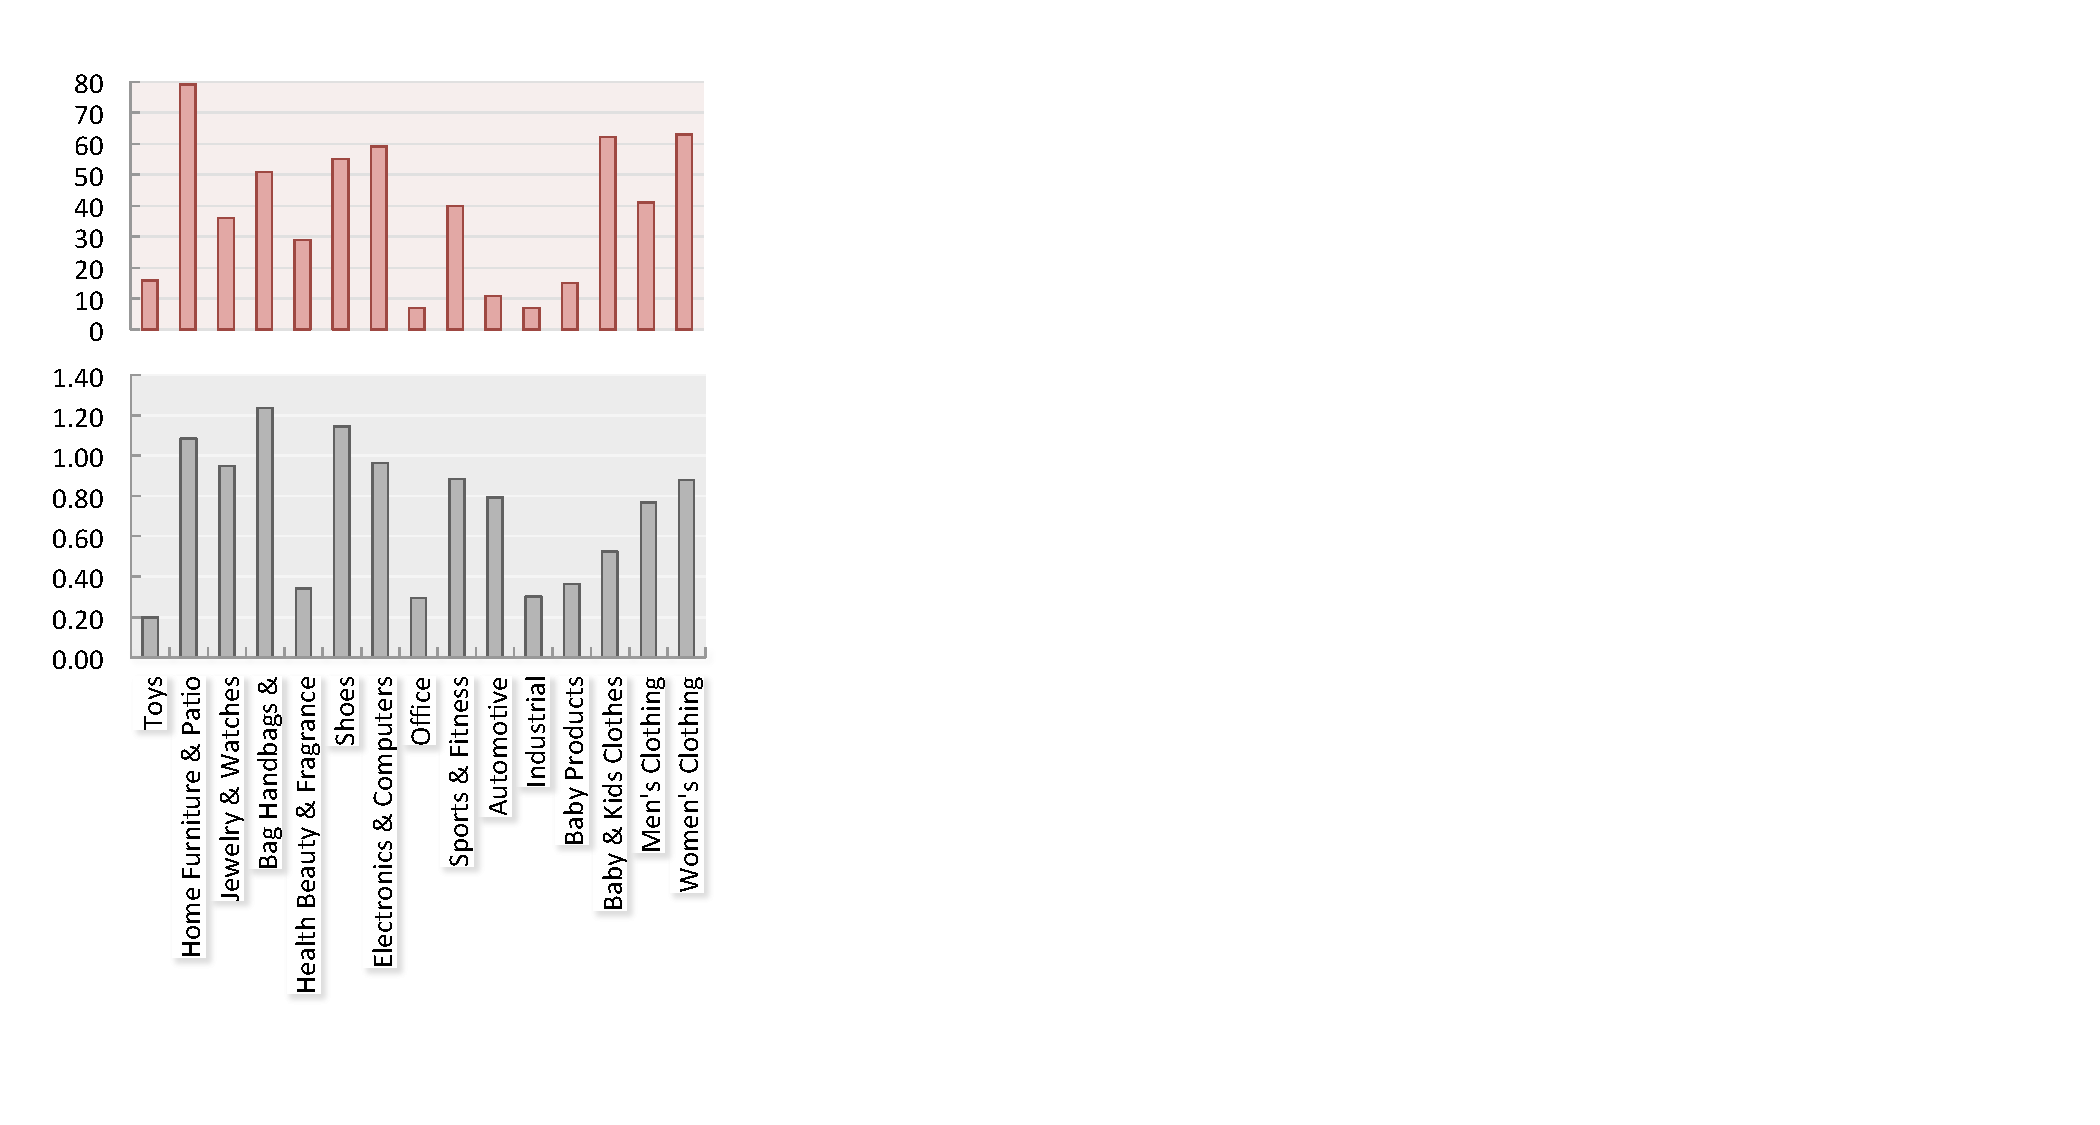
\includegraphics[width=0.26\textwidth]{images/BU2-branches+KL}}
	\vspace{-0.3cm}
	\caption{{\small Statistics on the datasets used for evaluation of classifiers: The top row shows the number of branches for a non-zero number of listings with titles for each dataset. The bottom row shows the KL divergence of the empirical distribution of listings in the branches in each subtree to the uniform distribution. These figures give us a rough measure of imbalance in each dataset. The mean KL divergence values are: BU1 dataset - 0.872; AmazonJulian dataset - 1.654; BU2 dataset - 0.715.}}
	\label{Fig:Dataset-statistics}
\end{figure}

An initial understanding of the imbalance in the datasets was important for us to judge expected generalization ability of several classifiers we experiment with. 
The top row in Fig. \ref{Fig:Dataset-statistics} shows the number of branches of level one taxonomy subtrees (i.e. class labels per level one category) for each of the datasets.
The AmazonJulian dataset (middle column) for taxonomy classification is the one obtained from \cite{Julian15}.
The dataset from BU1 shows the best kind of imbalance with a Pearson correlation coefficient of the total number of listings to number of branches in each of the subtrees to be 0.643.
This means that the number of branches in the subtrees correlate well with the volume of listings.
The AmazonJulian dataset (henceforth AmazonJ) \cite{Julian15}, show the highest number of branches in the subtrees on average.
This is possible since the extracted taxonomy may be a reflection of the navigational taxonomy which usually is listed in crawled product pages, instead of an internal data organization taxonomy.
However, for this dataset and that for BU2, the number of branches in the subtrees do not correlate well with the volume of listings indicating a much higher level of imbalance.

The bottom row of Fig. \ref{Fig:Dataset-statistics} shows the extra number of bits we would need to use to encode the listing distribution in the subtrees, if we thought the distribution was the uniform distribution i.e. balanced training set, but it was actually the empirical distribution.
The mean of the KL divergence values hint towards the fact that, on average, classifiers that are more or less resistant to imbalance should perform about the same for BU1 and BU2 datasets but perform significantly worse for the AmazonJ dataset under identical feature transformations (see Section \ref{Sect:results}).

An earlier work in this problem area has been well documented in \cite{Sun14} by Sun et al. 
The authors ... (gist of Chimera as it relates to our paper - specially Naive Bayes)

The main contributions of our work are three folds -- 
1) We conduct large scale experiments on taxonomy classification of product titles using state-of-the-art classifiers and conclude that the performances of GBTs and CNNs are much superior and comparable using only word unigram features which makes feature extraction very fast at runtime (Section \ref{Sect:results}). 
2) We make use of correspondence LDA models to identify patterns of data corruption in the training set that has been obtained from product page crawls in the wild (Section \ref{Subsect:BU2-noise-analysis}). 
3) We also show that including the list price and the root node of navigational breadcrumbs whenever available, boost prediction performance significantly.
